\documentclass{article}

% if you need to pass options to natbib, use, e.g.:
% \PassOptionsToPackage{numbers, compress}{natbib}
% before loading nips_2016
%
% to avoid loading the natbib package, add option nonatbib:
%\usepackage[nonatbib]{nips_2016}

%\usepackage{nips}

% to compile a camera-ready version, add the [final] option, e.g.:
\usepackage[final]{nips_2016}

\usepackage[utf8]{inputenc} % allow utf-8 input
\usepackage[T1]{fontenc}    % use 8-bit T1 fonts
\usepackage{hyperref}       % hyperlinks
\usepackage{url}            % simple URL typesetting
\usepackage{booktabs}       % professional-quality tables
\usepackage{amsfonts}       % blackboard math symbols
\usepackage{nicefrac}       % compact symbols for 1/2, etc.
\usepackage{microtype}      % microtypography

\usepackage{amssymb}
\usepackage{mathtools}
\usepackage{latexsym}
\usepackage{amsthm}
\usepackage{enumerate}
\usepackage{epsfig}
\usepackage{graphicx}
\usepackage{color}
\usepackage{float}
\usepackage{subfigure}
\usepackage{amsmath}
\usepackage{MnSymbol}
\usepackage{makeidx}
\usepackage{fancyhdr}
\usepackage{relsize}
\pagestyle{fancy}
\usepackage{lastpage}
\usepackage{url}
\usepackage{mathrsfs}

\newcommand{\F}{\ensuremath{\mathcal F}}
\DeclareMathSymbol{\R}{\mathbin}{AMSb}{"52}
\newcommand{\f}{\ensuremath{\mathcal f}}
\newcommand{\C}{\ensuremath{\mathcal C}}
\newcommand{\M}{\ensuremath{\mathcal M}}
\renewcommand{\H}{\ensuremath{\mathcal H}}
\newcommand{\pisys}{\ensuremath{\mathscr{L}}}
\newcommand{\lsys}[1]{\ensuremath{\lambda \lp #1 \rp}}
\newcommand{\A}{\ensuremath{\mathcal A}}
\newcommand{\E}{\ensuremath{\mathcal E}}
\renewcommand{\L}{\ensuremath{\mathcal L}}
\newcommand{\norm}[1]{\ensuremath{\mathcal \| #1 \|}}
\newcommand{\Exp}[1]{\ensuremath{\mathbb{E} \lb #1 \rb}}
\newcommand{\condExp}[2]{\ensuremath{\mathbb{E} \lb #1 | #2 \rb}}
\newcommand{\lp}{\ensuremath{\left(}}
\newcommand{\rp}{\ensuremath{\right)}}
\newcommand{\lb}{\ensuremath{\left[}}
\newcommand{\rb}{\ensuremath{\right]}}
\newcommand{\B}[1]{\ensuremath{\mathcal B\lp #1 \rp}}
\newcommand{\Pset}[1]{\ensuremath{\mathcal P\lp #1 \rp}}
\newcommand{\siga}[1]{\ensuremath{\sigma\lp #1 \rp}}
\newcommand{\Xrv}[1]{\ensuremath{X\lp #1 \rp}}
\newcommand{\Xrvi}[1]{\ensuremath{X \inv \lp #1 \rp}}
\newcommand{\Yrv}[1]{\ensuremath{Y\lp #1 \rp}}
\newcommand{\Prob}[1]{\ensuremath{\Pb\lp #1 \rp}}
\newcommand{\inv}{\ensuremath{^{-1}}}
\newcommand{\iprod}[2]{\ensuremath{\llangle #1, #2 \rrangle}}
\newcommand{\twopartdef}[4]
{
	\left\{
		\begin{array}{ll}
			#1 & \mbox{if } #2 \\
			#3 & \mbox{if } #4
		\end{array}
	\right.
}
\newcommand\independent{\protect\mathpalette{\protect\independenT}{\perp}}
\def\independenT#1#2{\mathrel{\rlap{$#1#2$}\mkern2mu{#1#2}}}

\title{Prior Formulation for Gaussian Process Hyperparameters}

% The \author macro works with any number of authors. There are two
% commands used to separate the names and addresses of multiple
% authors: \And and \AND.
%
% Using \And between authors leaves it to LaTeX to determine where to
% break the lines. Using \AND forces a line break at that point. So,
% if LaTeX puts 3 of 4 authors names on the first line, and the last
% on the second line, try using \AND instead of \And before the third
% author name.

\author{
  Rob Trangucci \\
  Applied Statistics Center\\
  Columbia University\\
  \texttt{robert.trangucci@gmail.com} 
  \and
  \textbf{Michael Betancourt} \\
  Applied Statistics Center \\
  Columbia University \\
  \texttt{betanalpha@gmail.com} 
  \and
  \textbf{Aki Vehtari} \\
  Department of Computer Science \\
  Aalto University \\
  \texttt{aki.vehtari@aalto.fi} 
  \and
  \textbf{Dan Simpson} \\
  Department of Statistics \\
  University of Toronto \\
  \texttt{dp.simpson@gmail.com} 
}

\begin{document}
% \nipsfinalcopy is no longer used

\maketitle

\begin{abstract}
  Gaussian processes (GP) are measures over functions, and as such, can be used
  as a rich prior for latent functions in Bayesian statistical models. However,
  the extreme flexibility of the prior requires weakly informative priors on GP
  hyperparameters. We develop a principled approach for specifying weakly
  informative priors for length scale hyperparameters that impose soft
  constraints on the space of functions represented by the Gaussian process
  prior.
\end{abstract}


\section{Introduction}

As noted by many authors (\citet{flaxman2015fast},
\citet{stein2012interpolation}, \citet{rasmussen2005gaussian},
\citet{fuglstad2015interpretable}), learning hyperparameters in Gaussian
process (GP) kernels is notoriously hard. The preponderance of literature has
focused estimating hyperparameters using marginal maximum likelihood for point
estimation (\citet{stein2012interpolation}, \citet{rasmussen2005gaussian},
\citet{warnes1987problems}), and the asymptotic properties of posterior
conditional mean functions in GP regressions (\citet{seeger2008information},
\citet{stein2012interpolation}, \citet{rasmussen2005gaussian},
\citet{williams2000upper}) with some exceptions such as
\citet{neal1998regression} and \citet{vanhatalo2013gpstuff}. As applied
statisticians, we face datasets with finitely many observations. As such there
will be many sets of hyperparameters that are consistent with our data; picking
any one set of them will lead to overfitting and poor out-of-sample
predictions. Instead, we advocate placing priors over hyperparameters and
integrate over our uncertainty when making predictions for new data. The
empirical advantage of full Bayesian inference versus point estimation are
well-documented (\citet{vehtariloo}). 
%% Add discussion of full-Bayes and MML theoretical considerations 
In order to do this we need to engineer principled priors that regularize the
Gaussian process sufficiently to admit practical fitting without compromising
its statistical utility. In this paper we'll investigate the consequences of
priors on hyperaparamters from theoretical and empirical perspectives, with a
focus on the finite data regime.

In order to gain insight into the empirical behavior of different priors, we
explore how efficiently 4 weakly informative priors can extract known
parameters in 12 different data generating processes, using techniques from
\citet{cook2012validation}. We deliberately chose to study a simple 1-D
Gaussian process regression model in order to avoid the increased complexities
of fitting a multi-dimensional GP.  Additionally, we aspire to develop a
coherent framework to choose weakly informative priors that can effectively
regularize nonidentifiabilities.  It is important to note that GPs in
higher-dimensional spaces will likely display different idiosyncrasies than
observed in the low-dimensional setting and these warrant further study.

In section \ref{background} we define the 1-D Gaussian process regression setting,
the hyperparameters of interest, and the mathematical basis for the manifestations
of weak identifiability in kernel hyperparameters. In section \ref{experiment}, we 
outline the experimental set up, and in section \ref{results} we discuss the results 
of our experiments. Stan code is presented in the appendix.


\section{Background} \label{background}

\subsection{Gaussian processes regression}

% Add definition of Matern kernel

The typical regression setting for a univariate response, $y$, as presented in \citet{flaxman2015fast},
$y_i \in \R, x_i \in \R^M\, i \in {1,\dots,n}$:
\begin{align*}
  \theta & \sim g(\phi) \\
  f(x) & \sim \text{GP}\lp \mu(x),
  K_\theta(x, x) \rp \\
  y_i & \sim \mathcal{N}\lp f(x_i), \delta \rp \forall i \\
\end{align*}
where $\text{GP}$ is a stochastic process from which finite-sample realizations are
multivariate Gaussian, and which is completely specified its mean vector $\mu$
and its covariance matrix $K_\theta(x, x)$. The $i, j$ th
element of $K_\theta(x, x)$:
\begin{align*}
  \text{cov}(f(x_i), f(x_j)) = k(x_i, x_j | \theta) 
\end{align*}
We focus on the exponentiated quadratic kernel, and the Mat\'{e}rn 5/2 kernel
where $\theta$ comprises two hyperparameters, $\ell$, the length-scale, and
$\alpha$, the marginal standard deviation. The exponentiated quadratic:
\begin{align} \label{kern_quad}
  k(x_i, x_j | \alpha, \ell) = \alpha^2 
\exp \left(
	- \dfrac{1}{2\ell^2} (x_{i} - x_{j})^2
\right)
\end{align}
%
The Mat\'{e}rn 5/2 kernel:
%
\begin{align} \label{kern_quad}
  k(x_i, x_j | \alpha, \ell) = \alpha^2 
	\left( 
	1 + \dfrac{\sqrt{5} |x_{i} - x_{j}}|{\ell} + \dfrac{5(x_{i} - x_{j})^2}{3\ell^2}
	\right)
	\exp \left(
	- \dfrac{\sqrt{5}{|x_{i} - x_{j}}}|{\ell} 
\right)
\end{align}
With $\ell$ and $\alpha$ fixed, inference of $f(x | \, \mathbf{y}, \theta)$ is
straightforward, with $f$ and $\mathbf{y}$ jointly normally distributed:
%put arrow above y and x to indicate vector of x and y $$:
\begin{align*} \begin{pmatrix} f\\ \mathbf{y} \\ \end{pmatrix} \sim
\mathcal{N} \lp \begin{pmatrix} \mathbf{0} \\ \mathbf{0} \end{pmatrix} ,\,\,
  \begin{pmatrix} K_\theta &
  K_\theta  \\ K_\theta &
  K_\theta + \delta ^ 2 \mathbf{I}\\ \end{pmatrix} \rp
\end{align*}
We can derive $p(f | \mathbf{y})$ from the properties of the conditional normal
distribution: 
\begin{align*}
  f \sim
  \mathcal{N}(K_\theta  (K_\theta + \delta ^ 2 \mathbf{I})^{-1}\mathbf{y},  
  K_\theta - K_\theta (K_\theta + \delta ^ 2 \mathbf{I})^{-1}K_\theta)
\end{align*}
Out-of-sample predictions are generated similarly:
\begin{align*} 
  \mathbf{\tilde{y}} \sim
  \mathcal{N}(&K_\theta(\mathbf{\tilde{x}},\mathbf{x}) (K_\theta(\mathbf{x},\mathbf{x}) +
  \delta ^ 2 \mathbf{I})^{-1}\mathbf{y},  
   \\ & K_\theta(\mathbf{\tilde{x}},\mathbf{\tilde{x}}) -K_\theta(\mathbf{\tilde{x}},\mathbf{x}) (K_\theta(\mathbf{x},\mathbf{x}) + \delta ^ 2 \mathbf{I})^{-1}K_\theta(\mathbf{x},\mathbf{\tilde{x}}) + \delta ^ 2 \mathbf{I})
\end{align*}
\begin{figure} \label{prior-lat-draws}
  \makebox[\textwidth]{\includegraphics[width=\textwidth,height=50mm]{plots/latent_draws_comparison.pdf}}
  \caption{Parameters which lead to expected zero crossings of 1/2 on left and 3.16 crossings on right} \label{prior-lat-draws}
\end{figure}
However, if we want to infer $\theta$ from the data we will need to take our
uncertainty in $\theta$ into account. We can see that both $\ell$ and $\alpha$
will impact our predictions for $\tilde{\mathbf{y}}$. $\alpha^2$ controls the
marginal variance of the stochastic process. For a fixed noise variance,
$\delta^2$, increasing the marginal variance of the stochastic process
increases the signal-to-noise ratio, $\alpha^2 / \delta^2$ (SN). $\ell$
controls the process's nonlinearity. Figure 1 shows the
difference between draws from a GP prior with a large $\ell$ and draws from a
GP prior with a small $\ell$.

Naturally, $\ell$ and $\alpha$ also control observable statistics of the
GP like the expected number of crossings of $f(x)$ on the interval $[0,
T]$ at level $u$, $\Exp{C_u}$. \citet{cramer2004stationary} show that $\Exp{C_u}$:
\begin{align*} 
  \Exp{C_u | \theta} = \dfrac{T}{\pi} 
\sqrt{-\dfrac{k_\theta^{\prime \prime}(0)}{k_\theta(0)}}
  \text{exp}\left(-\dfrac{u^2}{2k_\theta(0)}\right)
\end{align*} 
$\Exp{C_u | \theta}$ for the exponentiated quadratic kernel:
\begin{align*} 
  \Exp{C_u | \alpha, \ell} = \dfrac{T}{\pi \ell}\text{exp}\left(-\dfrac{u^2}{2 \alpha ^ 2} \right)
\end{align*} 
$\Exp{C_u | \theta}$ for the Mat\'{e}rn 5/2 kernel is:
% Add formula
We can see that at $u = 0$, we are left with $\Exp{C_u | \alpha, \ell} = T / \pi \ell$.  

However, at $u \neq 0$ $\alpha$ and $\ell$ are conflated in $\Exp{C_u | \alpha,
\ell}$.  This means that we would not be able to identify $\alpha$ and $\ell$
separately with number of crossings at different values of $u$.  This is an
inevitability of the parameterization of the exponentiated quadratic kernel,
and this feature of GPs can lead to problems when estimating $\alpha$ and
$\ell$ from data.

\subsection{Identifiability}

Identifiability is defined with respect to the equivalence of measures. If two
probability measures, $P_1$ and $P_2$ are equivalent, no amount of data can
differentiate between the two. If $P_\theta$ is a measure parameterized by
$\theta$, then there does not exist a consistent estimator for $\theta$
\citet{zhang2004inconsistent}.The identifiability of Gaussian processes depends
on the choice of kernel.  Estimators for length-scale and marginal standard
deviation in Mat\'{e}rn kernels are not consistent
\cite{zhang2004inconsistent}, but estimators for these same parameters are
weakly consistent in exponentiated quadratic covariance functions
\cite{abt1998fisher}. 

The concept of nonidentifiability does not exactly translate to Bayesian
inference. As long as we can define a proper posterior density, then we can
compute posterior expectations of parameters to yield posterior estimators of
parameters of interest. As noted by \cite{xie2004note}, defining a proper
posterior can be achieved by defining a proper prior. Thus it follows that if
we do not use a proper prior and have a classically nonidentified likelihood we
will not have a proper posterior. Running a Markov Chain Monte Carlo sampler
using the nonidentified model as our target density is fraught with danger
because Bayesian analysis must contend with all possible model configurations
consistent with the observed data. The sampler may have to explore an
infinitely diffuse posterior with infinite probability mass. When dealing with
a classically nonidentified model the challenge for a Bayesian analysis is to
use proper priors without limiting the model to configurations that don't fit
the data well while also accurately relfecting prior beliefs.

The non-identifiability of the Mat\'{e}rn presents a clear problem for Baysian
inference in that require proper priors. However, the fact that the
exponentiated quadratic kernel is the limit of the as Mat\'{e}rn $\nu
\rightarrow \infty$ will present problems for Bayesian inference, and will thus
also require carefully constructed priors. However, the flexibility of GPs
parameterized with the aforementioned kernels requires more than solely proper
priors to yield practically useful priors for inference when faced with sparse
data. This property is called ``weak identifiability''. We define the term and
discuss the finite data properties of both the Mat\'{e}rn 5/2 and the
exponentiated quadratic in the next two sections.

\subsubsection{Weak Identifiability}

With proper priors, weak identfiability is a function of both the model and the
observed, finite data at hand. For certain models and certain datasets, a
parameter in a model can be nearly nonidentified. That is, the prior has a
strong influence on the posterior. However, the data do contain some
information, however limited, as to the value of the hyperparameter. 
% is this next paragraph a fair statement?
In a model that is nonidentified like the GP parameterized with a Mat\'{e}rn
kernel, we might say that the posterior inference over $\ell$ and $\alpha$ are
solely properties of the prior. For instance the scale of the posterior for
both parameters are defined by the prior scale.

For models that are not classically nonidentified we can still observe behavior
in certain regions of the parameter space that resemble nonidentifiability,
namely extremely fat tails and basins of attraction at limits of the parameter
space.  We use the term ``weak identifiability'' to refer to a pathology
wherein parameters exhibit behavior consistent with classical
nonidentifiability in certain regions of parameter space. This is a property of
the joint prior and the likelihood. If the joint prior does not effectively
constrain the parameter space to a region where the likelihood is not flat,
then we say the model is weakly identied. 

This is not to be confused with the classical defintion of weak
identifiability, which is solely a characteristic of the statistical model.
Classical weak identfiability occurs when the asymptotic difference between two
estimates of the Fisher information, namely the variance of the score and the
negative expected value of the Hessian of the log-likelihood, does not converge
to zero \cite{andrews2015maximum}. The lack of convergence of the two measures
occurs for certain regions of the parameter space.

Guidance for a formal definition of weak identifiability can be found in Goel
et al.  (\cite{goel1981information}) which defines several information-based
measures of the gain in information about parameters after observing data. We
might consider measuring the KL-divergence of the marginal prior and the
marginal posterior, or of the joint-prior o 


\subsection{Weak identifiability in GPs}

% Show plot of likelihood profile vs. length-scale
% talk about data defining 

% Fake ridge for GP exponentiated quadratic
% ridge for exponential kernel

% plot prior vs. posterior for weakly identified

GPs on a fixed domain will always exhibit weak identifiability 
at length-scales that far exceed the scale of the data. This is
to be expected as the likelihood is essentially (what does essentially
mean?) flat (we should add some likelihood plots here). 

On the other hand, we must consider the spacing/design of our $x$ observations.
There is very little information in the data about what the process looks like
below the scale of the data. We necessarily are blind to the high-frequency 
(relative to the data spacing) properties of the GP.

In setting priors, we need to take an almost empircal Bayesian view and think
about how our GP is measured. 

\citet{rasmussen2005gaussian} show that a kernel $k(\boldsymbol{\tau})$ can
represented in the frequency domain by its Fourier transform:
\begin{align*}
  S(\mathbf{s}) = \int k(\mathbf{\tau}) \exp \left( -2 \pi i \mathbf{s}  \boldsymbol{\tau} \right) d\mathbf{s}
\end{align*}
The power spectrum for the exponentiated quadratic kernel can be derived analytically:
\begin{align*} 
  S(s) \propto \alpha^2 \ell
   \exp \left(
  - 2 \pi^2 \ell^2 s^2
\right)
\end{align*} 
This can be interpreted as the weight the kernel gives to an eigenfunction with
frequency $s$. Thus, for large $\ell$ the kernel gives more weight to low
frequency eigenfunctions and less weight to high-frequency eigenfunctions. 

We see problems with the spectrum of the kernel because both the $\alpha ^ 2$
term and the $\ell$ term scale the density $\exp \left(- 2 \pi^2 \ell^2 s^2
\right)$ term. In settings with sparse data and a low frequency signal,
increasing $\ell$ will force $S(s)$ to allocate more power to low frequency
signals at the expense of high frequency. Increasing $\alpha$ will allocate
more power to all frequencies, but because the data are sparse, we will not
have enough resolution to distinguish between an increase in $\alpha$ or an
increase in $\ell$. We can see that we will have the same problem with high
frequency signals and sparse data. As $\ell$ decreases, we allocate more power
to high-frequency functions at the expense of low-frequency functions. We can
decrease $\alpha$ in order to decrease the power allocated to all frequencies,
but the sparsity of the data necessarily means we will not be able to learn the
fine-resolution structure of the spectral density.

Note that the intuition provided above does not fit the definition of 
classical nonidentifiability; the spectral density certainly does change
values for two distinct sets of hyperparameters. However, sparse data
may not provide enough information to effectively constrain the hyperparameters.

There are also weak identification problems at the limits of the
hyperparameters' support. Turning to equation \ref{kern}, we can see that
the limiting behavior of the GP as $\ell \rightarrow \infty$ and $\alpha
\rightarrow 0$ each lead to the constant function. We can also see that $\ell
\rightarrow 0$ will conflate inferences in $\delta$.  Note that as $\ell
\rightarrow 0$ $\Exp{C_u | \alpha, \ell}$ diverges.

\section{Experiment} \label{experiment}

We investigate the properties of posterior inferences under several prior
formulations by generating 100 datasets for 12 data generating processes and
subsequently inferring $\alpha$, $\ell$, and $\delta$ by using Stan.

\subsection{Priors}

% Add GIG, talk about motivation for inverse gamma, compare
% gammas get rid of weibull. Leave 

Limiting behavior of GPs is an important driver of weak identifiability, so we
chose priors that differed in probability mass near zero and mass
in the tails of the densities, but that were similar in mass at other regions
of support. Thus, we calibrate our choices of priors for $\ell$ by fixing the
amount of probability mass between 0 and 1 for each prior at $\sim60\%$ but by
varying the priors' mass near zero and by varying the priors' tail heaviness.

This yields 4 priors: $\text{Gamma}(2, 2)$, $\text{Half-Cauchy}(0, 0.7)$,
$\text{Half-Normal}(0, 1.2)$, $\text{Weibull}(2, 1)$
\begin{figure}[t] 
  \makebox[\textwidth]{\includegraphics[width=\textwidth,height=70mm]{plots/prior_0_4_chart.pdf}}
  \caption{Priors over $\ell$ (length-scale)} \label{prior_plot}
\end{figure}
The $\text{Half-Cauchy}(0, 0.7)$ has the most mass at zero, and the most tail
mass. $\text{Gamma}(2, 2)$ has a heavy tail, but much lighter mass near zero
(in fact, it has zero mass exactly at zero, and thus is a zero-avoiding prior
\citet{gelman2014bayesian}). The $\text{Half-Normal}(0, 1.2)$ has a much
lighter tail than either the $\text{Half-Cauchy}(0, 0.7)$ or the
$\text{Gamma}(2, 2)$, but still has quite a bit of mass near zero.
$\text{Weibull}(2, 1)$ has about as much mass near zero as $\text{Gamma}(2, 2)$
but its tails are lighter than $\text{Half-Normal}(0, 1.2)$.

Another way to think about priors on length-scale is to consider the effective
number of parameters of a Gaussian process. The effective number of parameters
are the number of degrees of freedom for $f(x_i)$, the conditional mean of $y_i$:
$y_i \sim \mathcal{N}(f(x_i), \delta)$.
For example, a linear regression with one predictor and a mean has an effective
number of parameters of 2. If we exclude the predictor, we have 1 effective
parameter.
\begin{figure}[t] 
  \makebox[\textwidth]{\includegraphics[width=\textwidth,height=70mm]{plots/effective_number_parameter_zoomed.pdf}}
  \caption{Priors over the effective number of parameters of a linear smoother} \label{eff_pars_plot}
\end{figure}
\citet{rasmussen2005gaussian} show that for a GP the effective number of
parameters is:
\begin{align*}
  \text{tr}(K_\theta (K_\theta + \delta^2 I_n)^{-1})
\end{align*}
where $I_n$ is the $n$-dimensional identity matrix and tr is the sum of the
diagonal of a matrix. One should note that if we have a noiseless GP, our
effective number of parameters is $n$, which makes sense because if we do not
have noise in our process, our predicted mean at each data point $y_i$ is just
$y_i$. Thus, we would need $n$ parameters to model $n$ data points. In figure
\ref{eff_pars_plot}, we show 500 draws from the implied distribution for
effective number of parameters for all four of the priors. For each
distribution, we have fixed both $\alpha$ and $\delta$ at $0.71$. 

We can see that the Half-Cauchy distribution puts far more mass than the other
priors on small numbers of effective parameters. The Weibull generates a
more concentrated distribution than the other priors. We think that putting
priors in terms of effective number of parameters is a useful way to think
about priors on length-scale because the value can be anchored by effective
numbers of parameters in common classes of models.

We fix our priors for $\alpha$ and $\delta$ as $\text{Half-Normal}(0, 1)$. We
do not to vary the priors of $\alpha$ or $\delta$ because we believe that by
applying well-constructed priors to $\ell$ we can mitigate problems in
estimating $\alpha$. 

\subsection{Datasets}

% Add small data simulations, big data simulations
% for matern and 

We simulated 1000 datasets of 50 uniformly sampled data points on the domain
from $[-2, 2]$ from a Gaussian process regression for 12 sets of parameters.
The data generating processes vary in the severity of the nonlinearity in the
Gaussian process prior, induced by scaling $\ell$ from near $0.04$ to $2.54$.
We then generated two sets of 100 replicated datasets at each $\ell$, one set
which had a signal-to-noise ratio $\alpha ^ 2/ \delta ^ 2$ (SN) of $1$ and one
set which had a signal-to-noise ratio of $10$. The marginal variance $\alpha ^
2 + \delta ^ 2$ was fixed at 1 for each parameter set. The full data set
parameters are below:
\begin{table}[ht]
\centering
\caption{Data set parameters}
\begin{tabular}{rrrrrr}
  \hline
  & $\alpha$ & $\delta$ & SN & $\ell$ & $\Exp{C_0}$ \\ 
  \hline
1 & 0.71 & 0.71 & 1.00 & 2.54 & 0.50 \\ 
  2 & 0.95 & 0.30 & 10.00 & 2.54 & 0.50 \\ 
  3 & 0.71 & 0.71 & 1.00 & 1.27 & 1.00 \\ 
  4 & 0.95 & 0.30 & 10.00 & 1.27 & 1.00 \\ 
  5 & 0.71 & 0.71 & 1.00 & 0.64 & 2.00 \\ 
  6 & 0.95 & 0.30 & 10.00 & 0.64 & 2.00 \\ 
  7 & 0.71 & 0.71 & 1.00 & 0.40 & 3.16 \\ 
  8 & 0.95 & 0.30 & 10.00 & 0.40 & 3.16 \\ 
  9 & 0.71 & 0.71 & 1.00 & 0.13 & 10.00 \\ 
  10 & 0.95 & 0.30 & 10.00 & 0.13 & 10.00 \\ 
  11 & 0.71 & 0.71 & 1.00 & 0.04 & 31.62 \\ 
  12 & 0.95 & 0.30 & 10.00 & 0.04 & 31.62 \\ 
   \hline
\end{tabular}
\end{table}
\subsection{Inference}

We ran Stan on the command line (\citet{cmdstan}) for 1000 warmup and 1000
post-warmup iterations with 4 MCMC chains. All simulations run achieved
$\hat{R}$ < 1.05 for all parameters and achieved an acceptable effective sample
size, as suggested by \citet{gelman2014bayesian}.

\section{Results} \label{results}

We confirm our intuition that in settings with sparse data the tails of the
posterior distribution under heavy-tailed priors like the Cauchy are fat and
can lead to biased inferences. An instructive example arose from the setting in
which the signal-to-noise ratio was 1 and $\ell$ was set to 2.54 is worth
highlighting.

The data and the latent mean functions are nearly constant across the $[-2,2]$
interval, as shown in figure $\ref{gp_set_3}$. Our inferences for $\ell$ and $\alpha$
are plotted in figure \ref{gp_set_3_len}. The Cauchy model has clear problems ruling
out the constant function in its posterior. This has implications for the 
posterior predictive mean distribution, which was biased sharply towards
constant functions, as can be seen in figure \ref{gp_set_3_post_pred_cauchy}. The
posterior predictive mean distribution from the $\text{Half-Normal}(0, 1.2)$
prior over $\ell$ is better, though we can see the model still having trouble
distinguishing the true latent mean function. This is to be expected in settings
where the signal-to-noise ratio is low and the data are not informative.
\begin{figure}[htbp]
  \centering
  \makebox[\textwidth]{\includegraphics[width=\textwidth]{plots/dset_3_dgp.pdf}}
  \caption{Synthetic dataset with nearly constant latent function and high noise} \label{gp_set_3}
\end{figure}
\begin{figure}[htbp]
  \centering
  \makebox[\textwidth]{\includegraphics[width=\textwidth]{plots/dset_3_length_alpha.pdf}}
  \caption{Posterior distributions for $\ell$ and $\alpha$ under
  $\text{Half-Cauchy}(0, 0.7)$ and $\text{Half-Normal}(0, 1.2)$ priors for $\ell$} \label{gp_set_3_len}
\end{figure}
\begin{figure}[htbp]
  \centering
  \makebox[\textwidth]{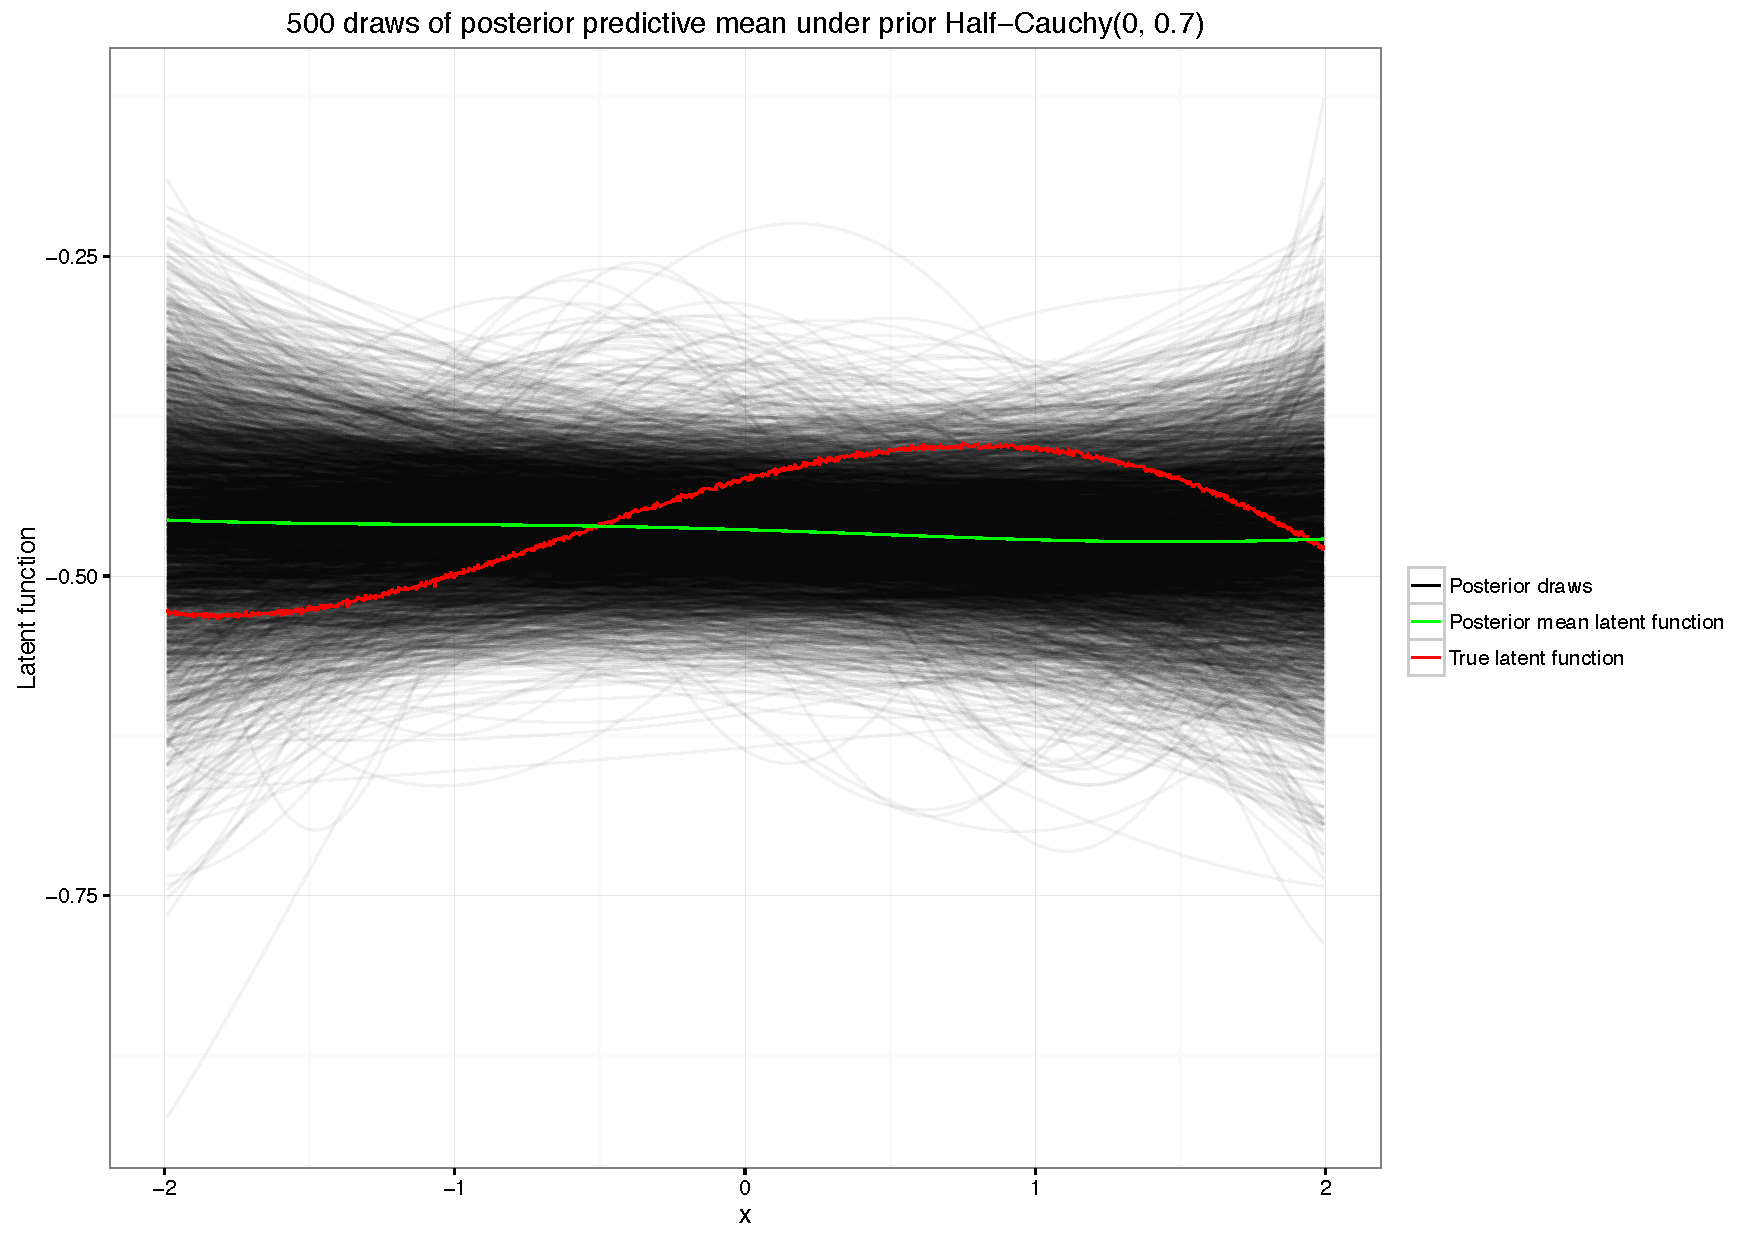
\includegraphics[width=\textwidth, height=75mm]{plots/half_cauchy_dset_3_post_pred_mean.pdf}}
  \caption{4000 draws from the distribution of the posterior predictive means for new data over the $[-2,2]$ domain} \label{gp_set_3_post_pred_cauchy}
\end{figure}
Given that the $\text{Half-Cauchy}(0, 0.7)$ has a heavy tail, and given that
constant GPs and GPs that are near-constant can be very hard to distinguish
using any one data set, we recommend against using the Cauchy when there are
clear practical upper bounds to $\ell$. The heavy tail of the Cauchy puts too
much mass on data generating processes that are indistinguishable from one
another using finite data sets.

This can be seen in the distribution of posterior means for $\ell$ and $\alpha$
across simulations in the low signal-to-noise, large $\ell$ scenario in figure \ref{joint_len_alpha}. 
\begin{figure}[htbp]
  \centering
  \makebox[\textwidth]{\includegraphics[width=\textwidth]{plots/dsets_2_5_alpha_0_7_alpha_length.pdf}}
  \caption{Posterior means of $\alpha$ and $\ell$. Data generated from GP with $\ell = 2.54, \alpha = 0.71, \delta = 0.71$.} \label{joint_len_alpha}
\end{figure}
We can see the fat tails of the Half-Cauchy leading to positively biased
estimates of length-scale in figure \ref{joint_len_alpha}. Given the paucity of
information in the data about the underlying mean function, our priors affect
the posterior mean estimates for $\ell$. This underscores the importance of
choosing weakly informative priors well. While the $\text{Half-Cauchy}(0, 0.7)$
allows for too much mass in the tail of the distribution, the
$\text{Weibull}(2, 1)$ has tails that are much too thin for the data generating
process, leading to estimates for length-scale that are negatively biased.

On the contrary, under the data generating processes that has a length-scale of
0.04 (with $\Exp{C_u | \alpha, \ell} = 31.62)$) and SN of 1, the posterior
means for $\ell$ are well-estimated by all priors, as can be seen in
\ref{joint_len_alpha_high_SN}. We had expected that priors with significant
mass near zero would have a hard time distinguishing between a length-scale of
zero and a length-scale greater than zero. However, this is likely a function
of the data being dense in $x$. We do see strong positive correlation between
$\ell$ and $\alpha$ in figure \ref{joint_len_alpha_high_SN}, which is a
byproduct of weak identifiability in the GP prior.
\begin{figure}[htbp]
  \centering
  \makebox[\textwidth]{\includegraphics[width=\textwidth]{plots/dsets_0_05_alpha_0_7_alpha_length.pdf}}
  \caption{Posterior means of $\alpha$ and $\ell$. Data generated from GP with $\ell = 0.04, \alpha = 0.71, \delta = 0.71$.} \label{joint_len_alpha_high_SN}
\end{figure}

We present tables for summary statistics from the experiments across the 100
replicated datasets in the Appendix. We computed the 50\% and 90\% interval
coverage, the bias, the mean interval width for $\alpha$ and $\ell$. The most
important takeaway is that if the tails of our priors are not constructed with
thought about the problem at hand, we can have low coverage, or high bias, no
matter the prior we use. 

\section{Conclusion}

We recommend against using a Cauchy density for a prior on the length-scale
hyperparameter $\ell$. In order to set an appropriate prior on length-scale,
the analyst should think about the expected number of effective parameters.
For example, compared to the other priors the Cauchy puts more mass on small
effective numbers of parameters. This may be why the GP with the
$\text{Half-Cauchy}(0, 0.7)$ had trouble distinguishing a signal in sparse
data. The Half-Cauchy prior also puts more mass than the other priors on large
effective numbers of parameters. The prior acts as a polarizing regularizer,
and will represent two potentially contradictory beliefs if the analyst is not
careful.

These experiments also suggest that setting a soft upper bound on $\ell$ by
using a prior on $\ell$ with a fast-decaying tail is a good weakly informative
prior.  More work needs to be done to understand joint priors over $\alpha$,
$\delta$, and $\ell$. Additionally, more work needs to be done on
reparameterizing the exponentiated quadratic kernel. Perhaps parameterizing the
kernel in terms of the effective number of parameters would more intuitive and
would not yield weak identifiability.

\pagebreak

\section{Appendix}

\subsection{Results details}

\subsubsection{Between simulation summaries: $\alpha$}

% latex table generated in R 3.3.0 by xtable 1.8-2 package
% Sun Dec  4 23:55:01 2016
\begin{table}[htbp]
\centering
\caption {Bias of posterior mean for $\alpha$} \label{bias_alpha} 
\begin{tabular}{rrrrrrrr}
  \hline
 & SN & $\ell$ & $\alpha$ & Cauchy & Normal & Weibull & Gamma \\ 
  \hline
1 & 1.00 & 0.04 & 0.71 & 0.02 & 0.03 & 0.03 & 0.03 \\ 
  2 & 1.00 & 0.13 & 0.71 & 0.06 & 0.06 & 0.07 & 0.06 \\ 
  3 & 1.00 & 0.40 & 0.71 & 0.09 & 0.10 & 0.12 & 0.11 \\ 
  4 & 1.00 & 0.64 & 0.71 & 0.13 & 0.15 & 0.15 & 0.15 \\ 
  5 & 1.00 & 1.27 & 0.71 & 0.08 & 0.07 & 0.02 & 0.06 \\ 
  6 & 1.00 & 2.54 & 0.71 & 0.06 & -0.05 & -0.09 & -0.05 \\ 
  7 & 10.00 & 0.04 & 0.95 & 0.00 & 0.00 & 0.00 & 0.00 \\ 
  8 & 10.00 & 0.13 & 0.95 & 0.01 & 0.01 & 0.02 & 0.02 \\ 
  9 & 10.00 & 0.40 & 0.95 & 0.07 & 0.07 & 0.09 & 0.08 \\ 
  10 & 10.00 & 0.64 & 0.95 & 0.10 & 0.11 & 0.12 & 0.11 \\ 
  11 & 10.00 & 1.27 & 0.95 & 0.02 & 0.02 & -0.02 & 0.01 \\ 
  12 & 10.00 & 2.54 & 0.95 & -0.00 & -0.11 & -0.19 & -0.10 \\ 
   \hline
\end{tabular}
\end{table}

\begin{table}[htbp]
\centering
\caption {50\% interval coverage for $\alpha$} \label{50_cover_alpha} 
\begin{tabular}{rrrrrrrr}
  \hline
 & SN & $\ell$ & $\alpha$ & Cauchy & Normal & Weibull & Gamma \\ 
  \hline
1 & 1.00 & 0.04 & 0.71 & 0.50 & 0.50 & 0.49 & 0.48 \\ 
  2 & 1.00 & 0.13 & 0.71 & 0.48 & 0.47 & 0.50 & 0.51 \\ 
  3 & 1.00 & 0.40 & 0.71 & 0.48 & 0.47 & 0.51 & 0.50 \\ 
  4 & 1.00 & 0.64 & 0.71 & 0.59 & 0.56 & 0.56 & 0.58 \\ 
  5 & 1.00 & 1.27 & 0.71 & 0.56 & 0.51 & 0.50 & 0.53 \\ 
  6 & 1.00 & 2.54 & 0.71 & 0.64 & 0.42 & 0.35 & 0.41 \\ 
  7 & 10.00 & 0.04 & 0.95 & 0.38 & 0.39 & 0.38 & 0.38 \\ 
  8 & 10.00 & 0.13 & 0.95 & 0.45 & 0.45 & 0.45 & 0.46 \\ 
  9 & 10.00 & 0.40 & 0.95 & 0.52 & 0.50 & 0.51 & 0.51 \\ 
  10 & 10.00 & 0.64 & 0.95 & 0.53 & 0.52 & 0.54 & 0.54 \\ 
  11 & 10.00 & 1.27 & 0.95 & 0.49 & 0.46 & 0.43 & 0.44 \\ 
  12 & 10.00 & 2.54 & 0.95 & 0.55 & 0.43 & 0.30 & 0.46 \\ 
   \hline
\end{tabular}
\end{table}

\begin{table}[htbp]
\centering
\caption {90\% interval coverage for $\alpha$} \label{90_cover_alpha} 
\begin{tabular}{rrrrrrrr}
  \hline
 & SN & $\ell$ & $\alpha$ & Cauchy & Normal & Weibull & Gamma \\ 
  \hline
1 & 1.00 & 0.04 & 0.71 & 0.83 & 0.82 & 0.83 & 0.83 \\ 
  2 & 1.00 & 0.13 & 0.71 & 0.85 & 0.85 & 0.85 & 0.83 \\ 
  3 & 1.00 & 0.40 & 0.71 & 0.90 & 0.90 & 0.90 & 0.89 \\ 
  4 & 1.00 & 0.64 & 0.71 & 0.88 & 0.85 & 0.87 & 0.86 \\ 
  5 & 1.00 & 1.27 & 0.71 & 0.93 & 0.92 & 0.89 & 0.95 \\ 
  6 & 1.00 & 2.54 & 0.71 & 0.93 & 0.92 & 0.87 & 0.91 \\ 
  7 & 10.00 & 0.04 & 0.95 & 0.85 & 0.86 & 0.85 & 0.87 \\ 
  8 & 10.00 & 0.13 & 0.95 & 0.84 & 0.84 & 0.86 & 0.86 \\ 
  9 & 10.00 & 0.40 & 0.95 & 0.88 & 0.88 & 0.90 & 0.88 \\ 
  10 & 10.00 & 0.64 & 0.95 & 0.89 & 0.90 & 0.91 & 0.91 \\ 
  11 & 10.00 & 1.27 & 0.95 & 0.97 & 0.97 & 0.93 & 0.95 \\ 
  12 & 10.00 & 2.54 & 0.95 & 0.98 & 0.91 & 0.82 & 0.90 \\ 
   \hline
\end{tabular}
\end{table}

\begin{table}[htbp]
\centering
\caption {90\% interval width for $\alpha$} \label{90_wid_alpha} 
\begin{tabular}{rrrrrrrr}
  \hline
 & SN & $\ell$ & $\alpha$ & Cauchy & Normal & Weibull & Gamma \\ 
  \hline
1 & 1.00 & 0.04 & 0.71 & 0.25 & 0.25 & 0.25 & 0.25 \\ 
  2 & 1.00 & 0.13 & 0.71 & 0.43 & 0.43 & 0.44 & 0.44 \\ 
  3 & 1.00 & 0.40 & 0.71 & 0.74 & 0.76 & 0.78 & 0.76 \\ 
  4 & 1.00 & 0.64 & 0.71 & 0.90 & 0.93 & 0.91 & 0.92 \\ 
  5 & 1.00 & 1.27 & 0.71 & 1.03 & 0.97 & 0.86 & 0.95 \\ 
  6 & 1.00 & 2.54 & 0.71 & 1.12 & 0.86 & 0.76 & 0.87 \\ 
  7 & 10.00 & 0.04 & 0.95 & 0.28 & 0.28 & 0.28 & 0.28 \\ 
  8 & 10.00 & 0.13 & 0.95 & 0.48 & 0.48 & 0.49 & 0.49 \\ 
  9 & 10.00 & 0.40 & 0.95 & 0.81 & 0.82 & 0.84 & 0.83 \\ 
  10 & 10.00 & 0.64 & 0.95 & 0.96 & 0.98 & 0.98 & 0.97 \\ 
  11 & 10.00 & 1.27 & 0.95 & 1.08 & 1.06 & 0.98 & 1.05 \\ 
  12 & 10.00 & 2.54 & 0.95 & 1.19 & 0.97 & 0.84 & 0.99 \\ 
   \hline
\end{tabular}
\end{table}

\subsubsection{Between simulation summaries: $\ell$}

\begin{table}[htbp]
\centering
\caption {Bias of posterior mean for $\ell$} \label{bias_ell} 
\begin{tabular}{rrrrrrr}
	 & SN & $\ell$ & Cauchy & Normal & Weibull & Gamma \\ 
  \hline
	1 & 1.00 & 0.04 & 0.00 & 0.00 & 0.00 & 0.00 \\ 
  2 & 1.00 & 0.13 & 0.01 & 0.01 & 0.01 & 0.01 \\ 
  3 & 1.00 & 0.40 & 0.03 & 0.03 & 0.05 & 0.04 \\ 
  4 & 1.00 & 0.64 & 0.13 & 0.14 & 0.14 & 0.14 \\ 
  5 & 1.00 & 1.27 & 1.15 & 0.10 & -0.07 & 0.07 \\ 
  6 & 1.00 & 2.54 & 2.95 & -0.66 & -1.09 & -0.64 \\ 
  7 & 10.00 & 0.04 & 0.00 & 0.00 & 0.00 & 0.00 \\ 
  8 & 10.00 & 0.13 & 0.00 & 0.00 & 0.00 & 0.00 \\ 
  9 & 10.00 & 0.40 & 0.01 & 0.01 & 0.02 & 0.01 \\ 
  10 & 10.00 & 0.64 & 0.02 & 0.03 & 0.04 & 0.03 \\ 
  11 & 10.00 & 1.27 & 0.09 & 0.06 & -0.02 & 0.04 \\ 
  12 & 10.00 & 2.54 & 0.50 & -0.46 & -0.87 & -0.42 \\ 
   \hline
\end{tabular}
\end{table}


\begin{table}[htbp]
\centering
\caption {50\% interval coverage for $\ell$} \label{50_cover_ell} 
\begin{tabular}{rrrrrrrr}
  \hline
 & SN & $\ell$ & $\alpha$ & Cauchy & Normal & Weibull & Gamma \\ 
  \hline
1 & 1.00 & 0.04 & 0.71 & 0.59 & 0.59 & 0.51 & 0.52 \\ 
  2 & 1.00 & 0.13 & 0.71 & 0.52 & 0.51 & 0.50 & 0.50 \\ 
  3 & 1.00 & 0.40 & 0.71 & 0.53 & 0.53 & 0.47 & 0.53 \\ 
  4 & 1.00 & 0.64 & 0.71 & 0.48 & 0.45 & 0.48 & 0.46 \\ 
  5 & 1.00 & 1.27 & 0.71 & 0.52 & 0.60 & 0.59 & 0.61 \\ 
  6 & 1.00 & 2.54 & 0.71 & 0.59 & 0.08 & 0.00 & 0.18 \\ 
  7 & 10.00 & 0.04 & 0.95 & 0.48 & 0.49 & 0.46 & 0.47 \\ 
  8 & 10.00 & 0.13 & 0.95 & 0.43 & 0.42 & 0.45 & 0.42 \\ 
  9 & 10.00 & 0.40 & 0.95 & 0.49 & 0.47 & 0.44 & 0.48 \\ 
  10 & 10.00 & 0.64 & 0.95 & 0.60 & 0.59 & 0.59 & 0.60 \\ 
  11 & 10.00 & 1.27 & 0.95 & 0.53 & 0.57 & 0.55 & 0.53 \\ 
  12 & 10.00 & 2.54 & 0.95 & 0.53 & 0.29 & 0.00 & 0.33 \\ 
   \hline
\end{tabular}
\end{table}

\begin{table}[htbp]
\centering
\caption {90\% interval coverage for $\ell$} \label{90_cover_ell} 
\begin{tabular}{rrrrrrrr}
  \hline
 & SN & $\ell$ & $\alpha$ & Cauchy & Normal & Weibull & Gamma \\ 
  \hline
1 & 1.00 & 0.04 & 0.71 & 0.90 & 0.90 & 0.88 & 0.89 \\ 
  2 & 1.00 & 0.13 & 0.71 & 0.88 & 0.88 & 0.86 & 0.88 \\ 
  3 & 1.00 & 0.40 & 0.71 & 0.95 & 0.95 & 0.91 & 0.94 \\ 
  4 & 1.00 & 0.64 & 0.71 & 0.88 & 0.87 & 0.86 & 0.86 \\ 
  5 & 1.00 & 1.27 & 0.71 & 0.96 & 0.98 & 0.98 & 0.98 \\ 
  6 & 1.00 & 2.54 & 0.71 & 0.98 & 0.82 & 0.02 & 0.84 \\ 
  7 & 10.00 & 0.04 & 0.95 & 0.87 & 0.87 & 0.82 & 0.86 \\ 
  8 & 10.00 & 0.13 & 0.95 & 0.87 & 0.87 & 0.88 & 0.88 \\ 
  9 & 10.00 & 0.40 & 0.95 & 0.88 & 0.88 & 0.89 & 0.89 \\ 
  10 & 10.00 & 0.64 & 0.95 & 0.94 & 0.94 & 0.93 & 0.93 \\ 
  11 & 10.00 & 1.27 & 0.95 & 0.94 & 0.94 & 0.96 & 0.94 \\ 
  12 & 10.00 & 2.54 & 0.95 & 0.92 & 0.85 & 0.16 & 0.86 \\ 
   \hline
\end{tabular}
\end{table}

\begin{table}[htbp]
\centering
\caption {90\% interval width for $\ell$} \label{90_wid_ell} 
\begin{tabular}{rrrrrrrr}
  \hline
 & SN & $\ell$ & $\alpha$ & Cauchy & Normal & Weibull & Gamma \\ 
  \hline
1 & 1.00 & 0.04 & 0.71 & 0.02 & 0.02 & 0.02 & 0.02 \\ 
  2 & 1.00 & 0.13 & 0.71 & 0.06 & 0.06 & 0.07 & 0.06 \\ 
  3 & 1.00 & 0.40 & 0.71 & 0.28 & 0.29 & 0.29 & 0.28 \\ 
  4 & 1.00 & 0.64 & 0.71 & 0.68 & 0.63 & 0.58 & 0.62 \\ 
  5 & 1.00 & 1.27 & 0.71 & 3.94 & 1.34 & 1.02 & 1.37 \\ 
  6 & 1.00 & 2.54 & 0.71 & 11.13 & 1.97 & 1.31 & 2.18 \\ 
  7 & 10.00 & 0.04 & 0.95 & 0.01 & 0.01 & 0.01 & 0.01 \\ 
  8 & 10.00 & 0.13 & 0.95 & 0.03 & 0.03 & 0.03 & 0.03 \\ 
  9 & 10.00 & 0.40 & 0.95 & 0.16 & 0.16 & 0.16 & 0.16 \\ 
  10 & 10.00 & 0.64 & 0.95 & 0.29 & 0.30 & 0.29 & 0.29 \\ 
  11 & 10.00 & 1.27 & 0.95 & 0.96 & 0.85 & 0.74 & 0.85 \\ 
  12 & 10.00 & 2.54 & 0.95 & 4.14 & 1.70 & 1.19 & 1.88 \\ 
   \hline
\end{tabular}
\end{table}

\pagebreak

\subsection{Stan code}

\begin{verbatim}
data {
  int<lower=1> D;
  int<lower=1> N;
  int<lower=1> N_pred;
  real x[N];
  vector[N] y;
  real x_pred[N_pred];
}
transformed data {
  vector[N] mu;
  matrix[N_pred, N_pred] nug_pred;

  mu = rep_vector(0, N);
  nug_pred = diag_matrix(rep_vector(1e-5,N_pred));
}
parameters {
  real<lower=0> length;
  real<lower=0> alpha;
  real<lower=0> delta;
}
model {
  matrix[N, N] L_Sigma;
  {
    matrix[N, N] Sigma;
    Sigma = cov_exp_quad(x, alpha, length);
    for (n in 1:N)
      Sigma[n, n] = Sigma[n,n] + square(delta);
    L_Sigma = cholesky_decompose(Sigma);
  }
  length ~ gamma(2, 2);
  delta ~ normal(0, 1);
  alpha ~ normal(0, 1);

  y ~ multi_normal_cholesky(mu, L_Sigma);
}
generated quantities {
  vector[N_pred] f_pred;

  {
    matrix[N, N] L_Sigma;
    vector[N] K_div_y;
    matrix[N, N_pred] k_x_x_pred;
    matrix[N, N_pred] v_pred;
    matrix[N_pred, N_pred] cov_f_pred;
    {
      matrix[N, N] Sigma;
      Sigma = cov_exp_quad(x, alpha, length);
      for (n in 1:N)
        Sigma[n, n] = Sigma[n,n] + square(delta);
      L_Sigma = cholesky_decompose(Sigma);
    }
    K_div_y = mdivide_left_tri_low(L_Sigma, y);
    K_div_y = mdivide_right_tri_low(K_div_y',L_Sigma)';
    k_x_x_pred = cov_exp_quad(x, x_pred, alpha, length);
    f_pred = k_x_x_pred' * K_div_y; 
    v_pred = mdivide_left_tri_low(L_Sigma, k_x_x_pred);
    cov_f_pred = cov_exp_quad(x_pred, alpha, length) - v_pred' * v_pred;

    f_pred = multi_normal_rng(f_pred, cov_f_pred + nug_pred);
  }
}
\end{verbatim}


\bibliographystyle{plainnat}
\bibliography{bib_inf_priors}

\end{document}
